\chapter{Modélisation des aimants}\label{annexe:ModelisationAimants}

Les aimants que nous avons utilisés sont composés d'un alliage de Niobium (Nb-Fe-B) et ont été achetés auprès de la société \nomofficiel{CALAMIT}. Ils se présentent sous la forme de parallélépipèdes rectangles de dimensions $L_a \times H_a \times P_a = 20 \times 10 \times 5$ mm avec une aimantation dirigée suivant la normale à la grande face. Nous avons modélisé ces aimants par des parallélépipèdes d'aimantation homogène. Une telle répartition volumique d'aimantation est rigoureusement équivalente à la présence d'une nappe de courant surfacique sur les faces latérales (voir figure~\nref{fig:AimantModel}). 
%
\bfigh
{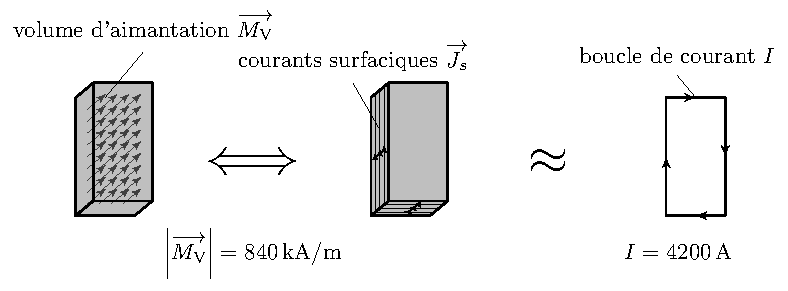
\includegraphics{P2/AimantModel}}
\CaptionFig{Modélisations d'un aimant. Le champ produit par nos aimants est proche de celui créé par une spire rectangulaire de même extension et parcourue par un courant de $\SI{4200}{\ampere}$.}
\label{fig:AimantModel}
\efigh

Le \chm produit par un aimant se calcule aisément, mais l'expression obtenue n'est pas simple:
\begin{equation}
	\Vecteur{B(\Vecteur{r})} =
\IntegraleBornes{\IntegraleBornes{\IntegraleBornes{
	-\frac{\mu_0}{4 \pi} 
	\Gradient{
		\frac{(\Vecteur{M_{\rm V}} \ddint^3 r_0) \cdot (\Vecteur{r}-\Vecteur{r_0})} {\Module{\Vecteur{r}-\Vecteur{r_0}}^3}
	}
}{}{-\frac{L_a}{2}}{\frac{L_a}{2}}
}{}{-\frac{H_a}{2}}{\frac{H_a}{2}}
}{}{-\frac{P_a}{2}}{\frac{P_a}{2}}
	\virguleformule
	\label{eq:AimantChampExacte}
\end{equation}
où on reconnaît sous le signe \termetech{intégrale} le \chm créé en $\Vecteur{r}$ par un dipôle élémentaire $(\Vecteur{M_{\rm V}} \ddint^3 r_0)$ placé en $\Vecteur{r_0}$. L'opérateur gradient $\Gradient{}$ porte sur la variable $\Vecteur{r}$. L'intégration s'effectue sur tout le volume de l'aimant.

Une modélisation moins \sotosay{sophistiqué} consiste à considérer l'aimant comme une simple boucle rectangulaire de courant (et non plus comme une nappe). On s'attend à ce que cette modélisation soit très proche de la précédente à partir du moment où l'on se place à une distance grande devant l'épaisseur de l'aimant. 
%L'expression du \chm est alors plus simple est vaut:
%\begin{equation}
%	sfsqdf = fqsdf vectoriel etc...
%	\label{eq:AimantChamp}
%\end{equation}

Afin de tester la fiabilité de cette modélisation pour nos aimants, nous avons effectué des mesures de \chm suivant l'axe passant par la grande face d'un aimant et perpendiculaire à celle-ci. La figure~\nref{fig:ChampAimant} témoigne d'un très bon accord avec cette modélisation d'aimantation uniforme ainsi qu'avec le modèle de spire rectangulaire. 
Ceci nous a permis en outre de déterminer l'aimantation $M_{\rm V} = \SI{840}{\kilo\ampere\per\meter}$ (qui est en bon accord avec l'aimantation nominale de \SI{800}{\kilo\ampere\per\meter}). 
%
\bfigh
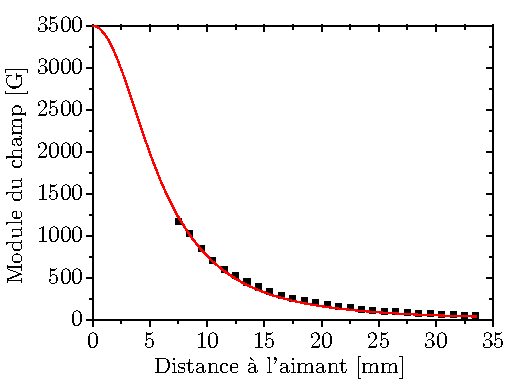
\includegraphics{P1/ChampAimant}
\CaptionFig{Mesure de la composante normale du \chm en fonction de la distance à la surface de l'aimant.}
\label{fig:ChampAimant}
\efigh


Il est intéressant de constater que le champ produit par un tel aimant est quasiment identique à celui créé par une spire rectangulaire de même extension et parcourue par un courant de $\SI{4200}{\ampere}$.

\Remarque{
Notons au passage qu'une aimantation pareille est assez remarquable. Pour s'en convaincre, considérons que:
\begin{itemize}
	\item dans un aimant (dont le volume est \SI{1}{\cubic{\centi\meter}}), il y a environ $\val{E23}$ atomes (le rayon covalent d'un atome de fer est d'environ \SI{2.3}{\angstrom}),
	\item le moment dipolaire magnétique d'un aimant est de $\SI{840}{\kilo\ampere\per\meter} \times \SI{1}{\cubic{\centi\meter}} = \SI{0,84}{\square\meter\ampere}$. 
\end{itemize}

Or ceci correspond environ au moment dipolaire magnétique obtenu si chaque atome de l'aimant est polarisé et apporte une contribution d'un magnéton de Bohr: $\val{E23} \times \muB = \val{E23} \times \val{9.27E-24} \approx \SI{0.93}{\square\meter\ampere}$. 
}
